\chapter{Definition und Konzepte}
Spring Security ist ein Sicherheit-Framework, welches sich in den Workflow des Spring J2EE Framework einf�gt, kann jedoch auch f�r andere Applikationen und Frameworks benutzt werden. Dieses Dokument beschr�nkt sich jedoch auf den Einsatz mit dem Spring Framework. Nahezu jede Komponente innerhalb des Frameworks kann man f�r den eigenen Gebrauch anpassen bzw. optimieren. Dadurch kann Spring Security mit sehr vielen anderen Authentisierungs-Komponenten zusammenarbeiten (z.B. SSO Authentications, eine grosse Vielfalt von Datenbanken usw...).

\section{Architektur}
Wenn ein HTTP-Request den Webserver trifft, kommt er zuerst in die sogenannte Filter-Chain. Diese Filter-Chain basiert auf den standard HTTP Servlet filter und ist der Eingangspunkt in die Applikation. Durch die Filter-Chain wird der Request an einen sogenannten \glqq Security Interceptor" weitergeleitet.  Der Security Interceptor authentisiert und authorisiert Requests auf Basis der Konfiguration und stellt Spring Informationen �ber die Authentisierung bereit.

\begin{figure}[h]{}
	\vspace{-0.8cm}
	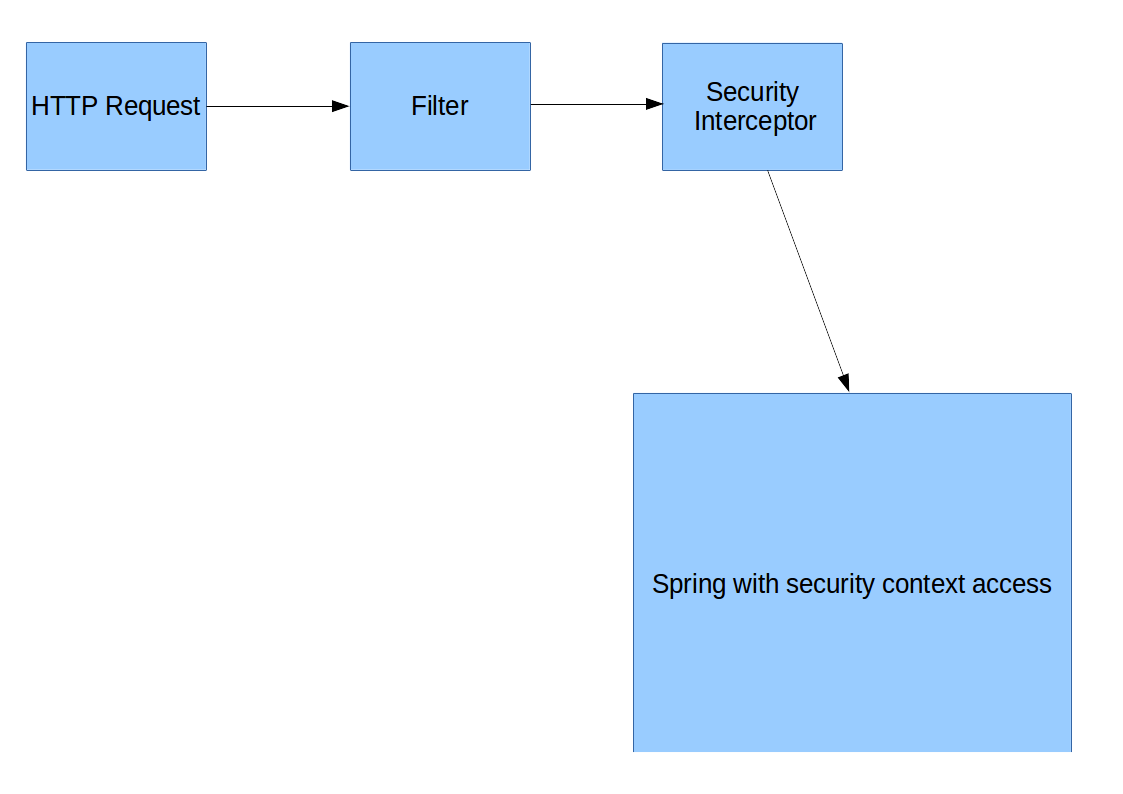
\includegraphics[width=0.8\textwidth]{Graphics/coreconcept.png}
	\caption{�bersicht Flow Spring Security, }
	\label{fig:coreconcept}
	\vspace{-0.7cm}
\end{figure}


\section{Spring Security Konzepte}
Spring benutzt verschiedene Komponenten um Benutzer zu authentisieren und zu autorisieren. Viele dieser Komponenten k�nnen benutzerdefiniert neu implementiert werden.
 \subsection{Core Klassen}
 Die Core Klassen dienen als Schnittstelle mit der Applikation und den Authentication und Autorisation Komponenten innerhalb von Springsecurity. Hier werden die eigentlichen sicherheitsrelevanten Informationen �ber die Anfrage abgespeichert (Authentication) und Abgerufen (Autorisation und Spring)
 
\subsubsection{SecurityContextHolder}
Der SecurityContextHolder besitzt alle Informationen �ber den Security Context f�r den jeweiligen Request. Innerhalb von Spring kann man �ber dieses Objekt alle Informationen �ber den User herausfinden. Zum Beispiel wird hier beschrieben wie der Username heisst, in welche Gruppe er sich befindet usw.

Dieses Objekt kann nicht benutzerdefiniert neu implementiert werden. 

Hier ein Beispiel wie man �ber den SecurityContextHolder den Username herausfindig machen kann.

\begin{lstlisting}
Object principal = SecurityContextHolder.getContext()
	.getAuthentication().getPrincipal();

if (principal instanceof UserDetails) {
  String username = ((UserDetails)principal).getUsername();
} else {
  String username = principal.toString();
}
\end{lstlisting}
\cite{springdoc}

\subsubsection{UserDetailService}
Der UserDetailService ist ein wichtiges Core-Interface in Spring Security. Es kann beliebig implementiert werden oder es k�nnen standart Implementationen von Spring Security gebraucht werden. Der UserDetailService dient als Bindeglied zwischen Spring Security und dem User-Store. Das Interface besteht aus genau einer Methode, welche einen String braucht und ein UserDetail Objekt zur�ckgibt: 
\begin{lstlisting}
  UserDetails loadUserByUsername(String username) throws
  	 UsernameNotFoundException;

\end{lstlisting}
\cite{springdoc}

Wenn die Authentisierung erfolgreich war, wird das UserDetail Objekt im SecurityContextHolder als Authentication eingepflegt. 

\subsubsection{GrantedAuthority}
Im SecurityContextHolder wird neben den UserDetails auch eine Autorit�t gespeichert. Man kann die Autorit�t mit getAuthority() aufrufen. Diese Autorit�t definiert Berechtigungen, welche der Benutzer hat. Normalerweise sind das Gruppen oder Rollen innerhalb der Applikation. Zum Beispiel w�re die Rolle "Admin" und "User", w�hrend die Admin Gruppe Berechtigungen zur Verwaltung der Applikation hat, hat der Benutzer die Berechtigung die Applikation zu benutzen. Spring Security kann aufgrund dieser Autorit�ten die Entscheidung treffen, ob die Anfrage berechtigt ist oder nicht. 

\subsection{Authentication}
Die Authentication Komponenten verifizieren die empfangenen Login-Informationen und erstellen eine Session. Die Securityinformationen werden anschliessend in einem Principal (siehe Core Components) abgespeichert und restlichen Komponenten in Spring Security sowie der Applikation zur Verf�gung gestellt.

\subsubsection{Was heisst Authentication in Spring?}
Bevor auf die verschiedenen Komponenten rund um Spring eingegangen werden kann, muss zuerst genau beschrieben werden, was Authentication im Kontext von Spring Security heisst.

Die Authentisierung beinhaltet folgenden T�tigkeiten:
\begin{itemize}
\item Der Benutzer ruft eine Webseite auf. 
\item Spring Security entscheidet ob die Webseite gesch�tzt ist oder nicht. 
\item Da der Benutzer noch nicht authentisiert ist, fragt Spring Security den Benutzer sich zu authentisieren 
\item Der Benutzer bekommt eine M�glichkeit seine Sicherheitsdetails einzugeben. (Dies Kann eine Username/Password Kombination sein (POST oder GET) , ein Zertifikat, eine Session oder etwas anderes)
\item Spring Security verifiziert die Korrektheit der bereitgestellten Informationen. (z.B. Spring Security pr�ft die gesendete Username/Password Kombination die gleiche ist, wie in der Datenbank abgelegt)
\item Falls die Informationen nicht korrekt sind, sendet Spring Security eine Access Denied Meldung zur�ck (Return Code 403)
\item Der Kontext des Users wird abgerufen. (z.b. die Rollen, Gruppen, Berechtigungen ...)
\end{itemize}

Alle T�tigkeiten danach werden nicht mehr zu Authentication zugerechnet, sondern zu Authorisation. 

\subsubsection{AuthenticationEntryPoint}
Der AuthenticationEntryPoint ist f�r die ersten drei Schritte zust�ndig. Er stellt somit den Eingangspunkt von anfragen an. Er kennt die Strategie, wohin weitergeleitet werden muss f�r noch nicht authentisierte User. Der AuthenticationEntryPoint kann man zus�tzlich selber Implementieren oder die Default-Implementation nutzen und diesen konfigurieren. 

\subsubsection{ExceptionTranslationFilter}
Access Denied Entscheidungen sind f�r Spring Security eine Exception. Der ExceptionTranslationFilter ist darum Verantwortlich, Access Denied Meldungen von dem AbstractSecurityInterceptor Interface (siehe Kapitel Autorisation) zu �bernehmen und eine Access Denied Meldung zu generieren (Schritt 6).

\subsubsection{UsernamePasswordAuthenticationToken}
Im vierten Schritt wird ein UsernamePasswordAuthenticationToken erstellt, welches die Sicherheitsdetails beinhaltet. Dieses Token wird weiter zum AuthenticationManager gesendet.

\subsubsection{AuthenticationManager}
Der AuthenticationManager checkt ob das usernamePasswordAuthenticationToken valid ist (Schritt 5) und erstellt daraus ein Authentication Objekt (Schritt 7) (siehe unter dem Kapitel Core). Dieses Authentication Objekt beinhaltet  anschliessen alles n�tige f�r eine korrekte Authentisierung. 

\subsubsection{SecurityContext zwischen Sessions}
Eine weitere wichtige Funktionalit�t ist das speichern des Users innerhalb einer Session. Der User sollte sich nicht jedes Mal neu authentisieren m�ssen wenn er auf einen anderen Link klickt. Auch dieses Feature kann man frei definieren. Als Standard wird jedoch ein sogenanntes \glqq JSESSIONID\grqq -Attribut mitgegeben, welches der Browser zur�cksendet. Diese Session wird im SecurityContextPersistance filter abgespeichert mit allen Informationen �ber den Authentisierten Benutzer.

\subsection{Autorisation}
Autorisation stellt eine Berechtigungskontrolle bereit. Da der User nun authentisiert ist, geht es bei der Autorisation um den Entscheid ob der User eine Berechtigung auf eine bestimmte Ressource hat. Die Klasse, welche diese Entscheidung vornimmt ist der \glqq AccessDecisionManager \grqq . Die Informationen, welcher der AccessDecisionManager braucht werden von dem SecurityInterceptor - ein Interface, welches wiederum implementiert werden kann - zusammengetragen. Folgendermassen wird dabei vorgegangen:
\begin{itemize}
\item Alle Konfigurations Attribute des Requests werden zusammengestellt
\item Die Ressource wird mit der Authentisierung und den Attributen zum AccessDecisionManager �bertragen, welcher anschliessend entscheidet ob die Berechtigung vorliegt.
\item Die Ressource wird ausgef�hrt oder es wird auf sie zugegriffen.
\item Der AfterInvocationManager wird ausgef�hrt nachdem die Ressource ausgef�hrt wurde.
\end{itemize}

\subsubsection{Konfigurations-Attribute}
Konfigurations-Attribute sind die ganzheitliche Konfiguration von Spring Security. Sie definieren was wo wie zugriff hat. Z.B. Welche Gruppe auf welche Ressourcen usw. Dies kann man in einer geschriebenen Konfiguration einprogrammieren oder einen eigenen SecurityInterceptor programmieren, der solche Konfigurations-Attribute definiert. 

\subsubsection{AfterInvocationManager}
Der AfterInvocationManager bildet das letzte Glied in der Kette der Autorisierung. Wenn z.B. der Access bis nach dem Methodenaufruf nicht sicher herausgefunden werden kann, so ist es dem AfterInvocationmanager m�glich, nach der Ausf�hrung der Ressource, das Ergebnis nochmal zu manipulieren und z.B. den Access revoken. 

